% !TEX program = xelatex
\documentclass[aspectratio=169]{beamer}
\usepackage{amsmath}
\usepackage{amssymb}
\usepackage{graphicx}
\usepackage{tcolorbox}
\usepackage{booktabs}
\usepackage{colortbl}
\usepackage{xcolor}
\usepackage{tikz}
\usetikzlibrary{intersections,decorations.pathreplacing,angles,quotes}
\usepackage[utf8]{inputenc}

% Custom colors
\definecolor{primary}{RGB}{41, 128, 185}
\definecolor{secondary}{RGB}{52, 152, 219}
\definecolor{accent}{RGB}{231, 76, 60}
\definecolor{lightgray}{RGB}{236, 240, 241}

% Theme customization
\usetheme{Madrid}
\usecolortheme{whale}
\setbeamercolor{structure}{fg=primary}
\setbeamercolor{background canvas}{bg=white}
\setbeamercolor{normal text}{fg=black}

% Title page info
\title{Pre-Calculus 11}
\subtitle{\textbf{6.2 Absolute Value Functions}}
\author{Created by Yi-Chen Lin}
\date{\today}

\begin{document}

% Title Page
\begin{frame}
    \titlepage
    \vfill
    \centering
    \footnotesize
\end{frame}

% Introduction
\begin{frame}{Graphing the Absolute Value of a Function}
    \begin{tcolorbox}[colback=lightgray,colframe=primary,title=Key Idea]
        \footnotesize
        When graphing $y=|f(x)|$, any point with a negative $y$-coordinate is reflected above the $x$-axis. Points with positive $y$-coordinates remain unchanged.
    \end{tcolorbox}
    \vspace{0.5em}
    \centering
    \textbf{Example:} $y = x - 2$ and $y = |x - 2|$
\end{frame}

% Example: Linear Function, Piecewise, and Its Absolute Value
\begin{frame}{Example: Linear Function and Its Absolute Value}
    \begin{columns}[T,onlytextwidth]
        \column{0.33\textwidth}
        \textbf{Original:} $y = x - 2$
        \begin{tikzpicture}[scale=0.7]
            \draw[->] (-1,0) -- (5,0) node[right] {$x$};
            \draw[->] (0,-3) -- (0,3) node[above] {$y$};
            \draw[thick,primary] (-0.5,-2.5) -- (4,2);
            \foreach \x/\y in {0/-2, 1/-1, 2/0, 3/1, 4/2} {
                \filldraw[accent] (\x,\y) circle (2pt);
            }
        \end{tikzpicture}
        \column{0.34\textwidth}
        \textbf{Piecewise:}
        \[
        y = \begin{cases} x-2, & x \geq 2 \\ -(x-2), & x < 2 \end{cases}
        \]
        \column{0.33\textwidth}
        \textbf{Absolute Value:} $y = |x - 2|$
        \begin{tikzpicture}[scale=0.7]
            \draw[->] (-1,0) -- (5,0) node[right] {$x$};
            \draw[->] (0,-0.5) -- (0,3) node[above] {$y$};
            \draw[thick,primary] (2,0) -- (4,2);
            \draw[thick,primary] (2,0) -- (0,2);
            \foreach \x/\y in {0/2, 1/1, 2/0, 3/1, 4/2} {
                \filldraw[accent] (\x,abs(\x-2)) circle (2pt);
            }
        \end{tikzpicture}
    \end{columns}
\end{frame}

% Steps to Find Piecewise Function for Parabola
\begin{frame}{Steps to Find Piecewise Function for $|$Parabola$|$}
    \begin{tcolorbox}[colback=lightgray,colframe=primary,title=How to Write the Piecewise Function]
        \footnotesize
        \begin{enumerate}
            \item \textbf{Find the $x$-intercepts} of the parabola by setting $y=0$ and solving for $x$. Use these intercepts to split the domain into (Left, Middle, Right).
            \item \textbf{Write the equation inside the absolute value} for each domain interval, \textbf{without} the absolute value sign.
            \item \textbf{Graph the parabola} and indicate which parts are below the $x$-axis (these will be flipped up).
            \item For the part(s) that were flipped, \textbf{place a negative sign in front of the entire equation} (with brackets) for those intervals.
        \end{enumerate}
    \end{tcolorbox}
\end{frame}

% Parabola Example (Reformatted, scale 0.3)
\begin{frame}{Example: Parabola and Its Absolute Value}
    \begin{tcolorbox}[colback=lightgray,colframe=primary,title=Reflecting Below the X-axis]
        \footnotesize
        To graph $y = |f(x)|$ for a parabola, reflect any part below the $x$-axis upward.
    \end{tcolorbox}
    \vspace{0.5em}
    \begin{columns}[T,onlytextwidth]
        \column{0.65\textwidth}
        \centering
        \begin{tikzpicture}[scale=0.3]
            % Axes
            \draw[->] (-8,0) -- (8,0) node[right] {$x$};
            \draw[->] (0,-8) -- (0,12) node[above] {$y$};
            % Parabola above x-axis (red)
            \draw[thick,red,domain=-4:4,samples=100] plot (\x,{8-0.5*\x*\x});
            % Parabola below x-axis (blue, dashed)
            \draw[thick,blue,dashed,domain=-8:-4,samples=50] plot (\x,{8-0.5*\x*\x});
            \draw[thick,blue,dashed,domain=4:8,samples=50] plot (\x,{8-0.5*\x*\x});
            % Reflected part (blue, solid)
            \draw[thick,blue,domain=-8:-4,samples=50] plot (\x,{-8+0.5*\x*\x});
            \draw[thick,blue,domain=4:8,samples=50] plot (\x,{-8+0.5*\x*\x});
            % Intersection points
            \filldraw[black] (-4,0) circle (8pt);
            \filldraw[black] (4,0) circle (8pt);
        \end{tikzpicture}
        \column{0.35\textwidth}
        \begin{tcolorbox}[colback=white,colframe=accent,title=Explanation]
            \footnotesize
            \textcolor{blue}{Blue dashed:} Original part below $x$-axis\\
            \textcolor{blue}{Blue solid:} Reflected upward\\
            \textcolor{red}{Red:} Original part above $x$-axis (unchanged)
        \end{tcolorbox}
    \end{columns}
\end{frame}

% Example: Quadratic Function, Piecewise, and Its Absolute Value
\begin{frame}{Example: Quadratic Function and Its Absolute Value}
    \begin{columns}[T,onlytextwidth]
        \column{0.33\textwidth}
        \textbf{Original:} $y = x^2 - 3$
        \begin{tikzpicture}[scale=0.7]
            \draw[->] (-3,0) -- (3,0) node[right] {$x$};
            \draw[->] (0,-4) -- (0,6) node[above] {$y$};
            \draw[thick,primary,domain=-2:2,samples=100] plot (\x,{\x*\x-3});
            \foreach \x in {-2,-1,0,1,2} {
                \filldraw[accent] (\x,{\x*\x-3}) circle (2pt);
            }
        \end{tikzpicture}
        \column{0.34\textwidth}
        \textbf{Piecewise:}
        \[
        y = \begin{cases} x^2-3, & |x| \geq \sqrt{3} \\ -(x^2-3), & |x| < \sqrt{3} \end{cases}
        \]
        \column{0.33\textwidth}
        \textbf{Absolute Value:} $y = |x^2 - 3|$
        \begin{tikzpicture}[scale=0.7]
            \draw[->] (-3,0) -- (3,0) node[right] {$x$};
            \draw[->] (0,-0.5) -- (0,6) node[above] {$y$};
            % Above x-axis
            \draw[thick,primary,domain=-1.732:1.732,samples=100] plot (\x,{3-\x*\x});
            \draw[thick,primary,domain=-2:-1.732,samples=50] plot (\x,{\x*\x-3});
            \draw[thick,primary,domain=1.732:2,samples=50] plot (\x,{\x*\x-3});
            \foreach \x in {-2,-1,0,1,2} {
                \filldraw[accent] (\x,{abs(\x*\x-3)}) circle (2pt);
            }
        \end{tikzpicture}
    \end{columns}
\end{frame}

% Example: Cubic Function, Piecewise, and Its Absolute Value
\begin{frame}{Example: Cubic Function and Its Absolute Value}
    \begin{columns}[T,onlytextwidth]
        \column{0.33\textwidth}
        \textbf{Original:} $y = x^3 - 2x$
        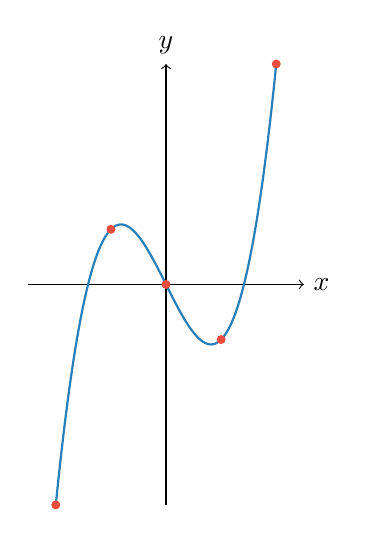
\begin{tikzpicture}[scale=0.7]
            \draw[->] (-2.5,0) -- (2.5,0) node[right] {$x$};
            \draw[->] (0,-4) -- (0,4) node[above] {$y$};
            \draw[thick,primary,domain=-2:2,samples=100] plot (\x,{\x*\x*\x-2*\x});
            \foreach \x in {-2,-1,0,1,2} {
                \filldraw[accent] (\x,{\x*\x*\x-2*\x}) circle (2pt);
            }
        \end{tikzpicture}
        \column{0.34\textwidth}
        \textbf{Piecewise:}
        \[
        y = \begin{cases} x^3-2x, & x^3-2x \geq 0 \\ -(x^3-2x), & x^3-2x < 0 \end{cases}
        \]
        \column{0.33\textwidth}
        \textbf{Absolute Value:} $y = |x^3 - 2x|$
        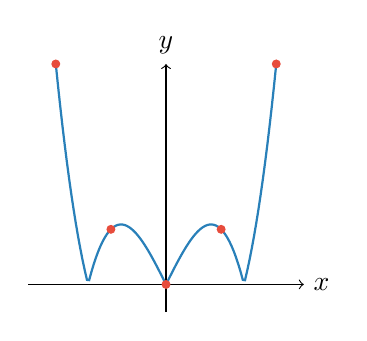
\begin{tikzpicture}[scale=0.7]
            \draw[->] (-2.5,0) -- (2.5,0) node[right] {$x$};
            \draw[->] (0,-0.5) -- (0,4) node[above] {$y$};
            \draw[thick,primary,domain=-2:2,samples=100] plot (\x,{abs(\x*\x*\x-2*\x)});
            \foreach \x in {-2,-1,0,1,2} {
                \filldraw[accent] (\x,{abs(\x*\x*\x-2*\x)}) circle (2pt);
            }
        \end{tikzpicture}
    \end{columns}
\end{frame}

% Practice: Graph and Analyze
\begin{frame}{Practice: Graph and Analyze}
    \begin{tcolorbox}[colback=lightgray,colframe=accent,title=Practice]
        \footnotesize
        Graph $y = |x^2 - 4|$ and:
        \begin{enumerate}
            \item Determine the $x$- and $y$-intercepts
            \item State the domain and range
            \item Write the piecewise function
        \end{enumerate}
    \end{tcolorbox}
\end{frame}

% Multiple Choice: Piecewise
\begin{frame}{Multiple Choice: Piecewise Function}
    \begin{tcolorbox}[colback=lightgray,colframe=primary,title=Which is the correct piecewise function for $y=|x^2-4|$?]
        \footnotesize
        \begin{enumerate}
            \item $y = x^2-4$ for $x \leq -2$ or $x \geq 2$; $y = -(x^2-4)$ for $-2 < x < 2$
            \item $y = x^2-4$ for $x < 0$; $y = -(x^2-4)$ for $x \geq 0$
            \item $y = x^2-4$ for $x > 0$; $y = -(x^2-4)$ for $x \leq 0$
        \end{enumerate}
    \end{tcolorbox}
\end{frame}

% Practice Problem 1
\begin{frame}{Practice: Graph the Absolute Value}
    \begin{tcolorbox}[colback=lightgray,colframe=accent,title=Practice 1]
        \footnotesize
        Graph $y = |x + 1|$.
    \end{tcolorbox}
\end{frame}

% Practice Problem 2
\begin{frame}{Practice: Graph the Absolute Value}
    \begin{tcolorbox}[colback=lightgray,colframe=accent,title=Practice 2]
        \footnotesize
        Graph $y = |-2x + 3|$.
    \end{tcolorbox}
\end{frame}

% Practice Problem 3
\begin{frame}{Practice: Graph the Absolute Value}
    \begin{tcolorbox}[colback=lightgray,colframe=accent,title=Practice 3]
        \footnotesize
        Graph $y = |x^2 - 2|$.
    \end{tcolorbox}
\end{frame}

% Practice Problem 4
\begin{frame}{Practice: Graph the Absolute Value}
    \begin{tcolorbox}[colback=lightgray,colframe=accent,title=Practice 4]
        \footnotesize
        Graph $y = |-x^2 + 4|$.
    \end{tcolorbox}
\end{frame}

% Practice Problem 5
\begin{frame}{Practice: Graph the Absolute Value}
    \begin{tcolorbox}[colback=lightgray,colframe=accent,title=Practice 5]
        \footnotesize
        Graph $y = |x^2 - 4x + 3|$.
    \end{tcolorbox}
\end{frame}

\end{document} 